\documentclass{beamer}
\usetheme{metropolis}           % Use metropolis theme

\usepackage{tikz}
\usepackage[utf8]{inputenc}
\usepackage[spanish]{babel}

\usepackage{smartdiagram}
\usepackage{qtree}
\usepackage{verbatim}
\usepackage{svg}
\usepackage{graphicx}
\usepackage{color}
\definecolor{lightgray}{rgb}{0.95, 0.95, 0.95}
\definecolor{darkgray}{rgb}{0.4, 0.4, 0.4}
%\definecolor{purple}{rgb}{0.65, 0.12, 0.82}
\definecolor{editorGray}{rgb}{0.95, 0.95, 0.95}
\definecolor{editorOcher}{rgb}{1, 0.5, 0} % #FF7F00 -> rgb(239, 169, 0)
\definecolor{editorGreen}{rgb}{0, 0.5, 0} % #007C00 -> rgb(0, 124, 0)
\definecolor{orange}{rgb}{1,0.45,0.13}		
\definecolor{olive}{rgb}{0.17,0.59,0.20}
\definecolor{brown}{rgb}{0.69,0.31,0.31}
\definecolor{purple}{rgb}{0.38,0.18,0.81}
\definecolor{lightblue}{rgb}{0.1,0.57,0.7}
\definecolor{lightred}{rgb}{1,0.4,0.5}
\usepackage{upquote}
\usepackage{listings}
\lstset{language=html,
	basicstyle=\footnotesize\ttfamily,
	keywordstyle=\footnotesize\color{blue}\ttfamily,
}

%\usebackgroundtemplate%
%{%
%	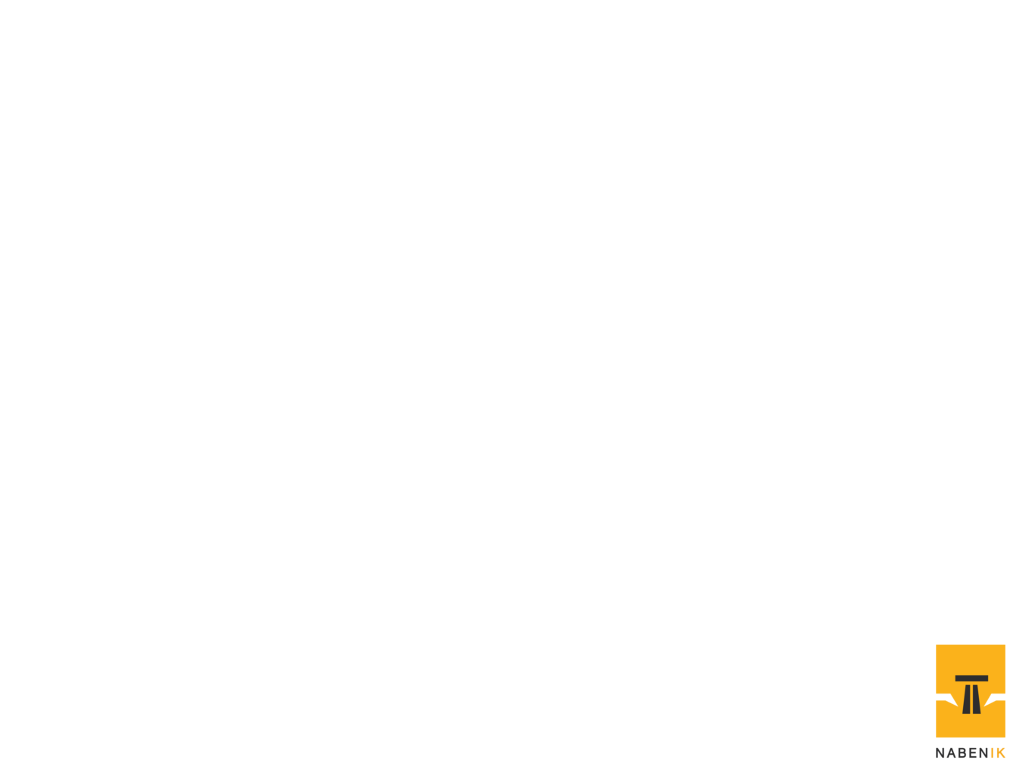
\includegraphics[width=\paperwidth]{Images/fondo}%
%}
\title{Introducción a JakartaEE 8}
\author{Víctor Orozco - @tuxtor}
\institute{Hackdays comunidad hispana 2018}
\date{\today}

\begin{document}

\frame{\titlepage}

\begin{frame}{Acerca de}
\begin{figure}
	\centering
	
\includegraphics[width=\linewidth]{Images/fescudos}
\end{figure}
\end{frame}

\begin{frame}{Acerca de}
\huge @guatejug  @jakartaEE @payara\_fish @EventosJEspanol @MedellinJug :)
\end{frame}



\section{JavaEE 7}
\begin{frame}{Framework - Ecosistema}
	\begin{figure}
		\centering
		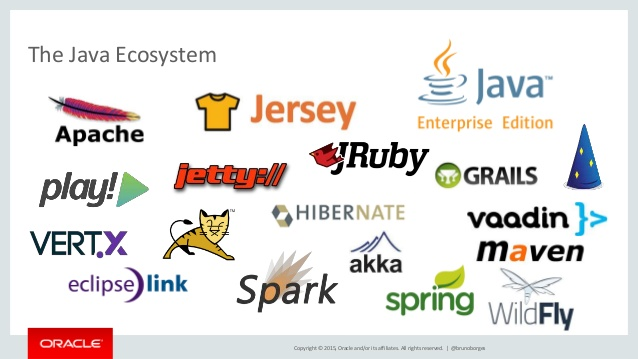
\includegraphics[width=0.9\linewidth]{Images/ecosystem}
	\end{figure}
\end{frame}

\begin{frame}{Framework - Enterprise}
	\begin{figure}
		\centering
		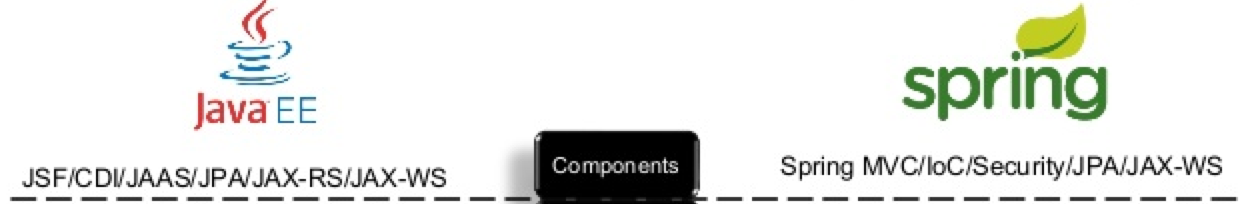
\includegraphics[width=\linewidth]{Images/javaeesp}
	\end{figure}
\end{frame}

\begin{frame}{JavaEE 7}
	\begin{figure}
		\centering
		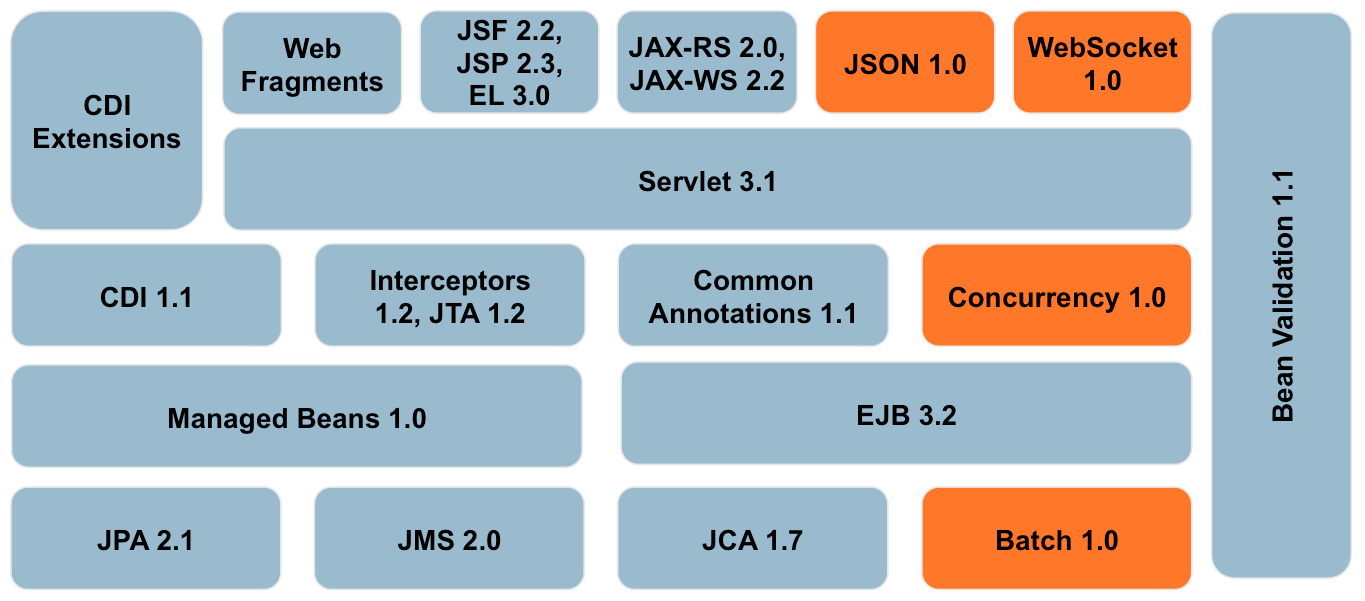
\includegraphics[width=0.9\linewidth]{Images/javaee7-pancake.png}
	\end{figure}	
\end{frame}

\begin{frame}{JavaEE 7}
	\begin{itemize}
		\item API Rest - JAX-RS 2.0
		\item WebSocket - WebSocket 1.0, Servlet 3.1
		\item JSON - JSON API 1.0
		\item SOA, Microservices
	\end{itemize}
	\begin{figure}
		\centering
		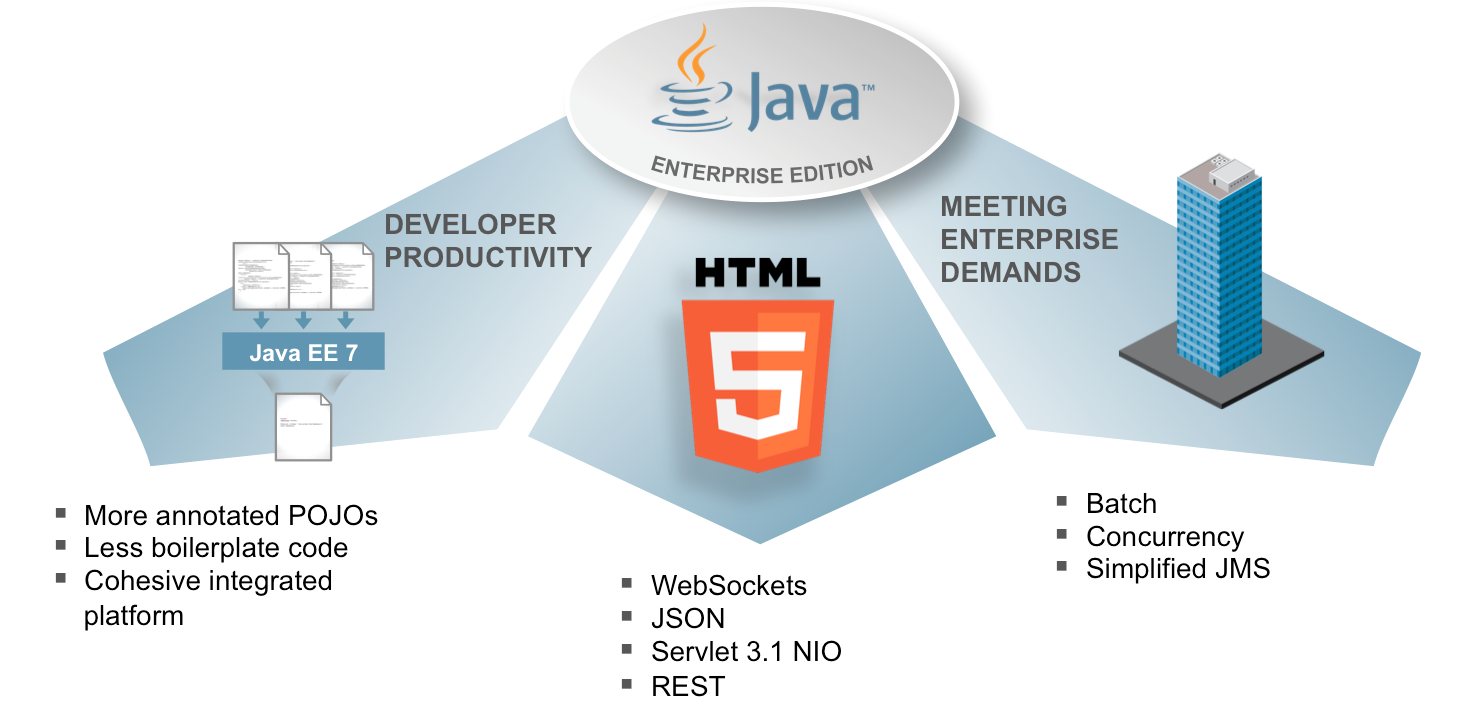
\includegraphics[width=0.65\linewidth]{Images/javaee7-theme}
	\end{figure}
\end{frame}

\section{Revisión de conceptos}

\begin{frame}{Arquitecturas enterprise}
\begin{itemize}
	\item ORM
	\item Persistence Entity
	\item DAO/Repository
	\item CDI
	\item Endpoint
	\item REST
	\item SPA
\end{itemize}
\end{frame}


\begin{frame}{Arquitecturas enterprise}
\begin{itemize}
	\item ORM - Framework de cambio de paradigma (Relacional-POO)
	\item Persistence Entity - Entidad que representa una o varias tablas
	\item DAO/Repository - Unidad a cargo de la persistencia de una o varias entidades
	\item CDI - Inyección de dependencia y contexto
	\item Endpoint - Unidad a cargo de comunicaciones con el exterior
	\item REST - Protocolo de comunicación de datos via HTTP
	\item SPA - Aplicación elaborada con HTML5, JavaScript y CSS 3 que interactua unicamente para solicitar datos
\end{itemize}
\end{frame}

\begin{frame}{Arquitecturas enterprise}
\begin{itemize}
	\item ORM - JPA
	\item Persistence Entity - JPA Entity
	\item DAO/Repository - EJB, Managed Bean
	\item CDI - Managed Beans
	\item Endpoint - JAX-RS
	\item REST - JAX-RS + JSON Provider
	\item SPA - AngularJS
\end{itemize}
\end{frame}

\begin{frame}{Demo}
Java EE HOL

\url{https://github.com/comunidad-hispana-jugs/workshop-03-JEE8_-_JSE10}

\end{frame}



%TODO

\section{JavaEE 8, EE4J}

\begin{frame}{JavaEE 8}
\begin{figure}
	\centering
	
\includegraphics[width=0.6\linewidth]{Images/futuro}
\end{figure}
\end{frame}

\begin{frame}{JavaEE 8}
\begin{figure}
	\centering
	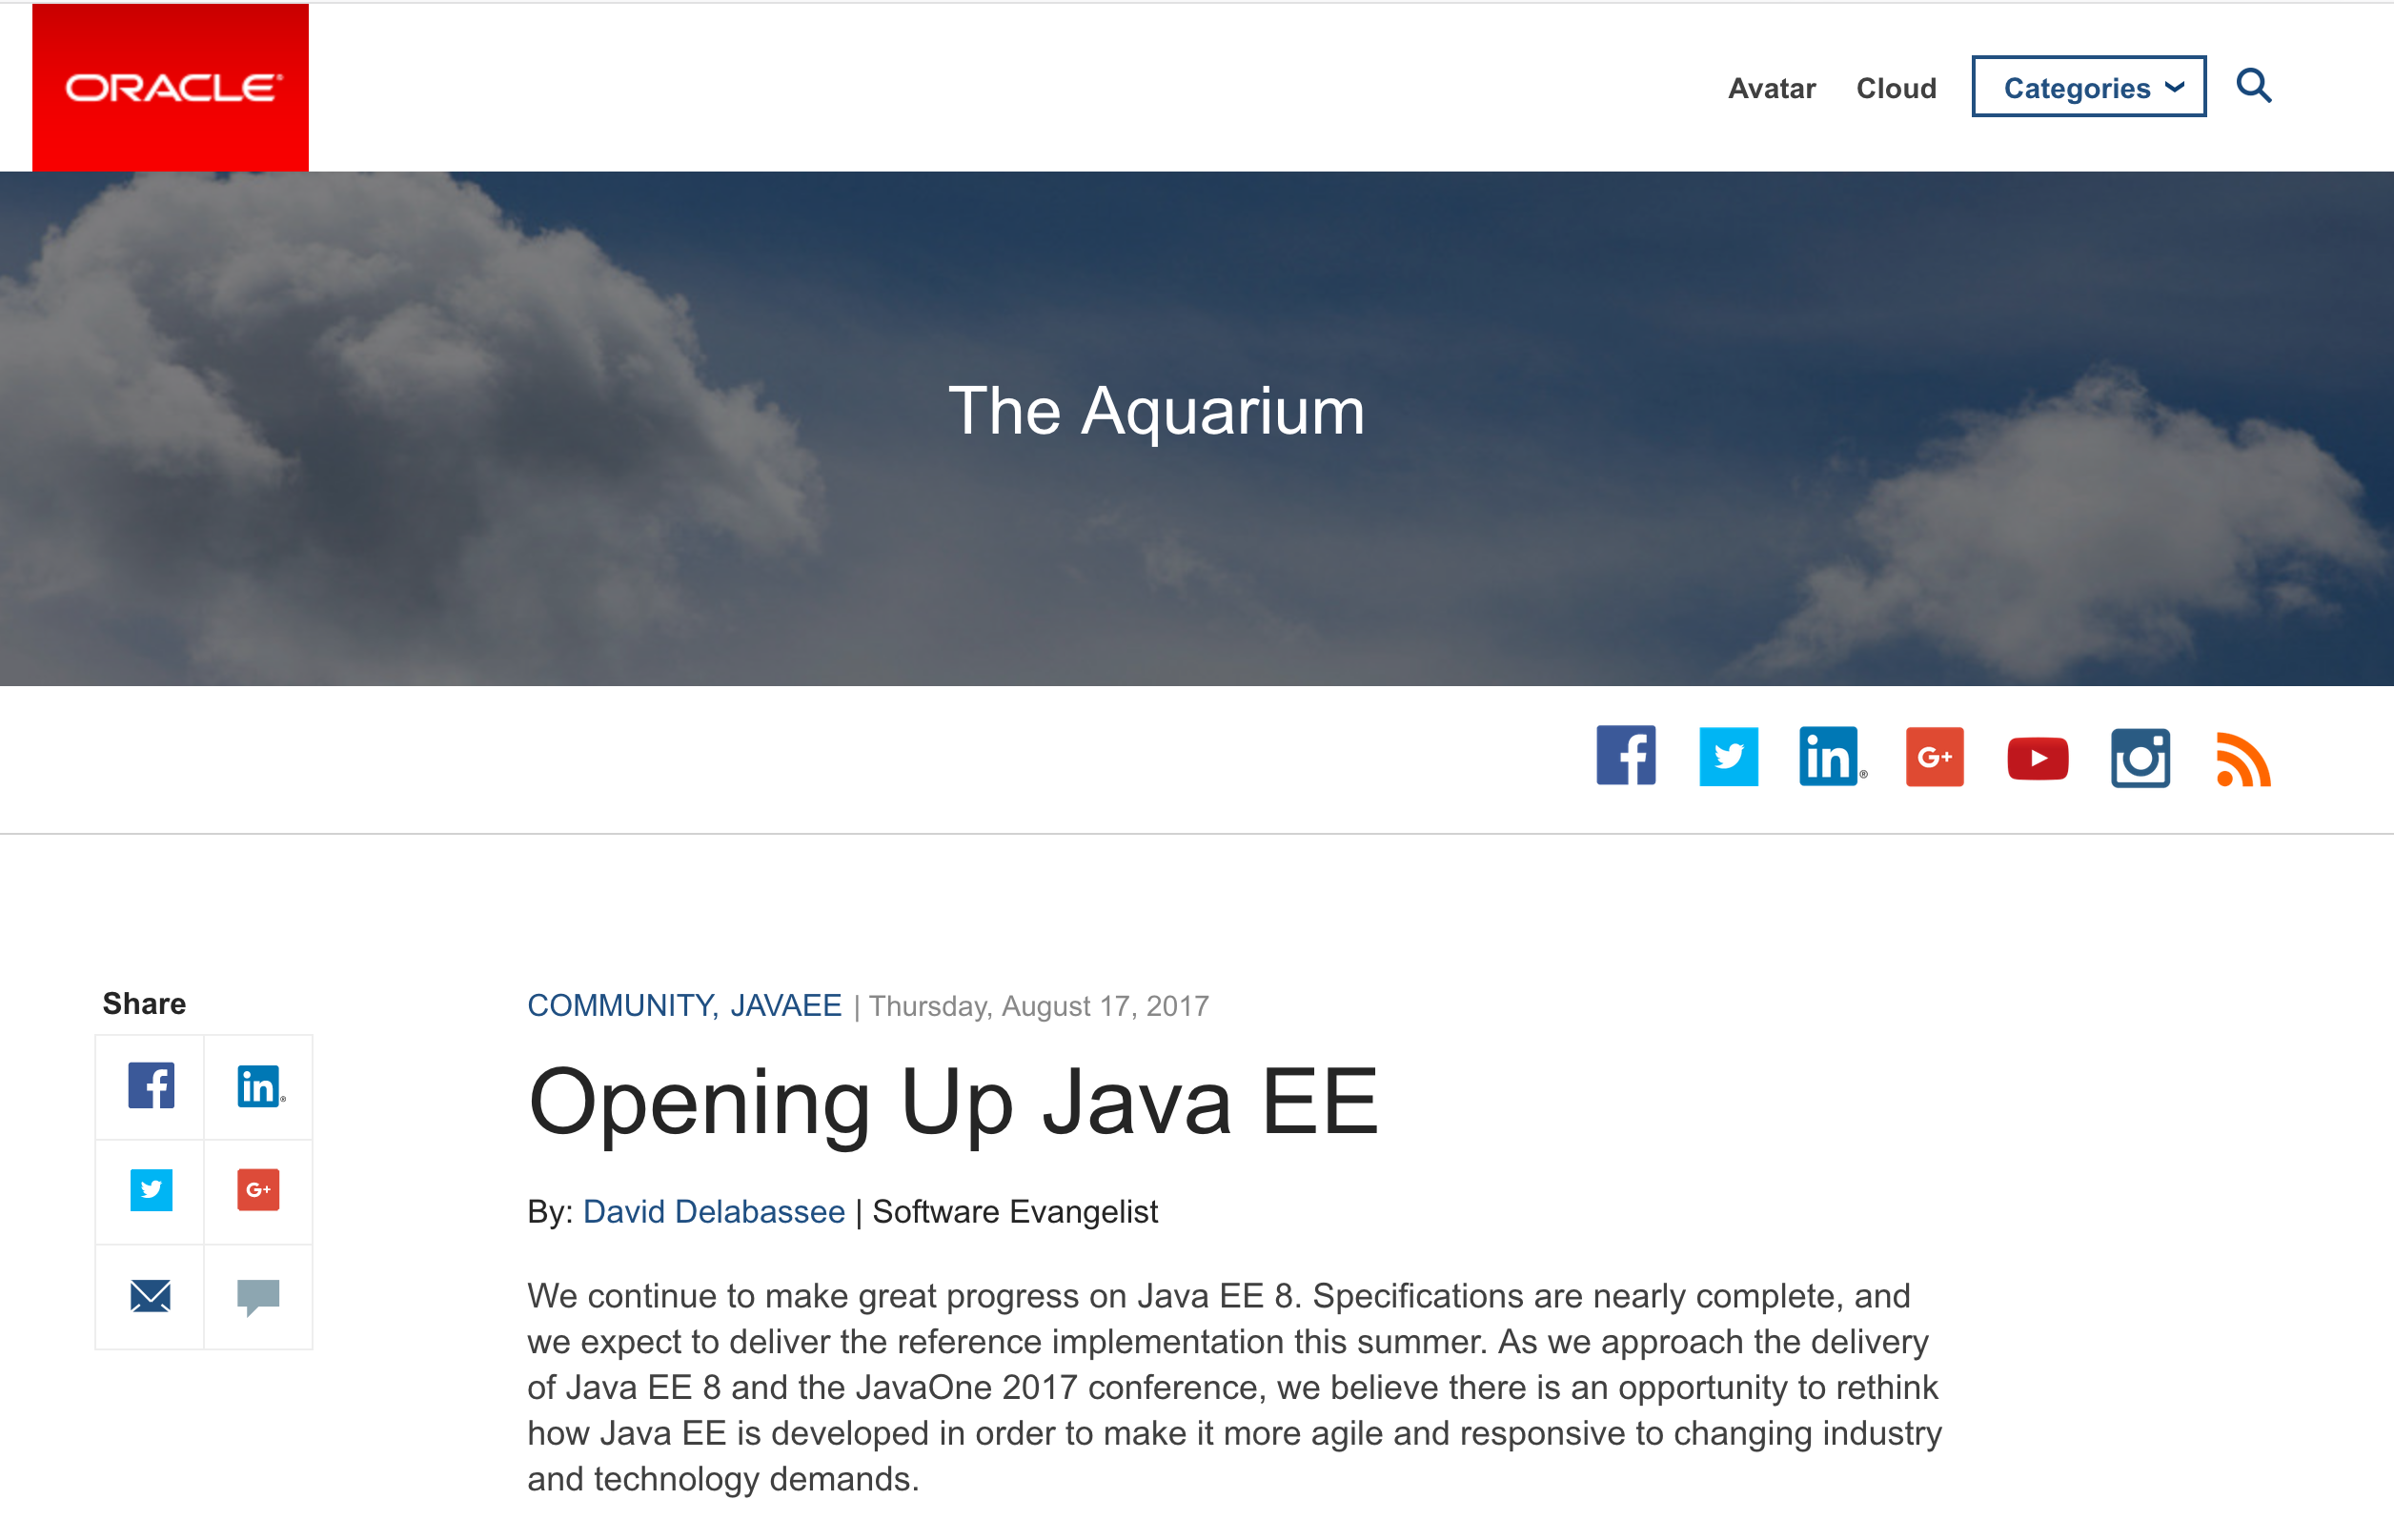
\includegraphics[width=\linewidth]{Images/javaeeopen}
\end{figure}
\end{frame}


\begin{frame}{JavaEE 8}
\begin{figure}
	\centering
	
\includegraphics[width=\linewidth]{Images/payara5}
\end{figure}
\end{frame}


\begin{frame}{JavaEE 8}
\begin{figure}
	\centering
	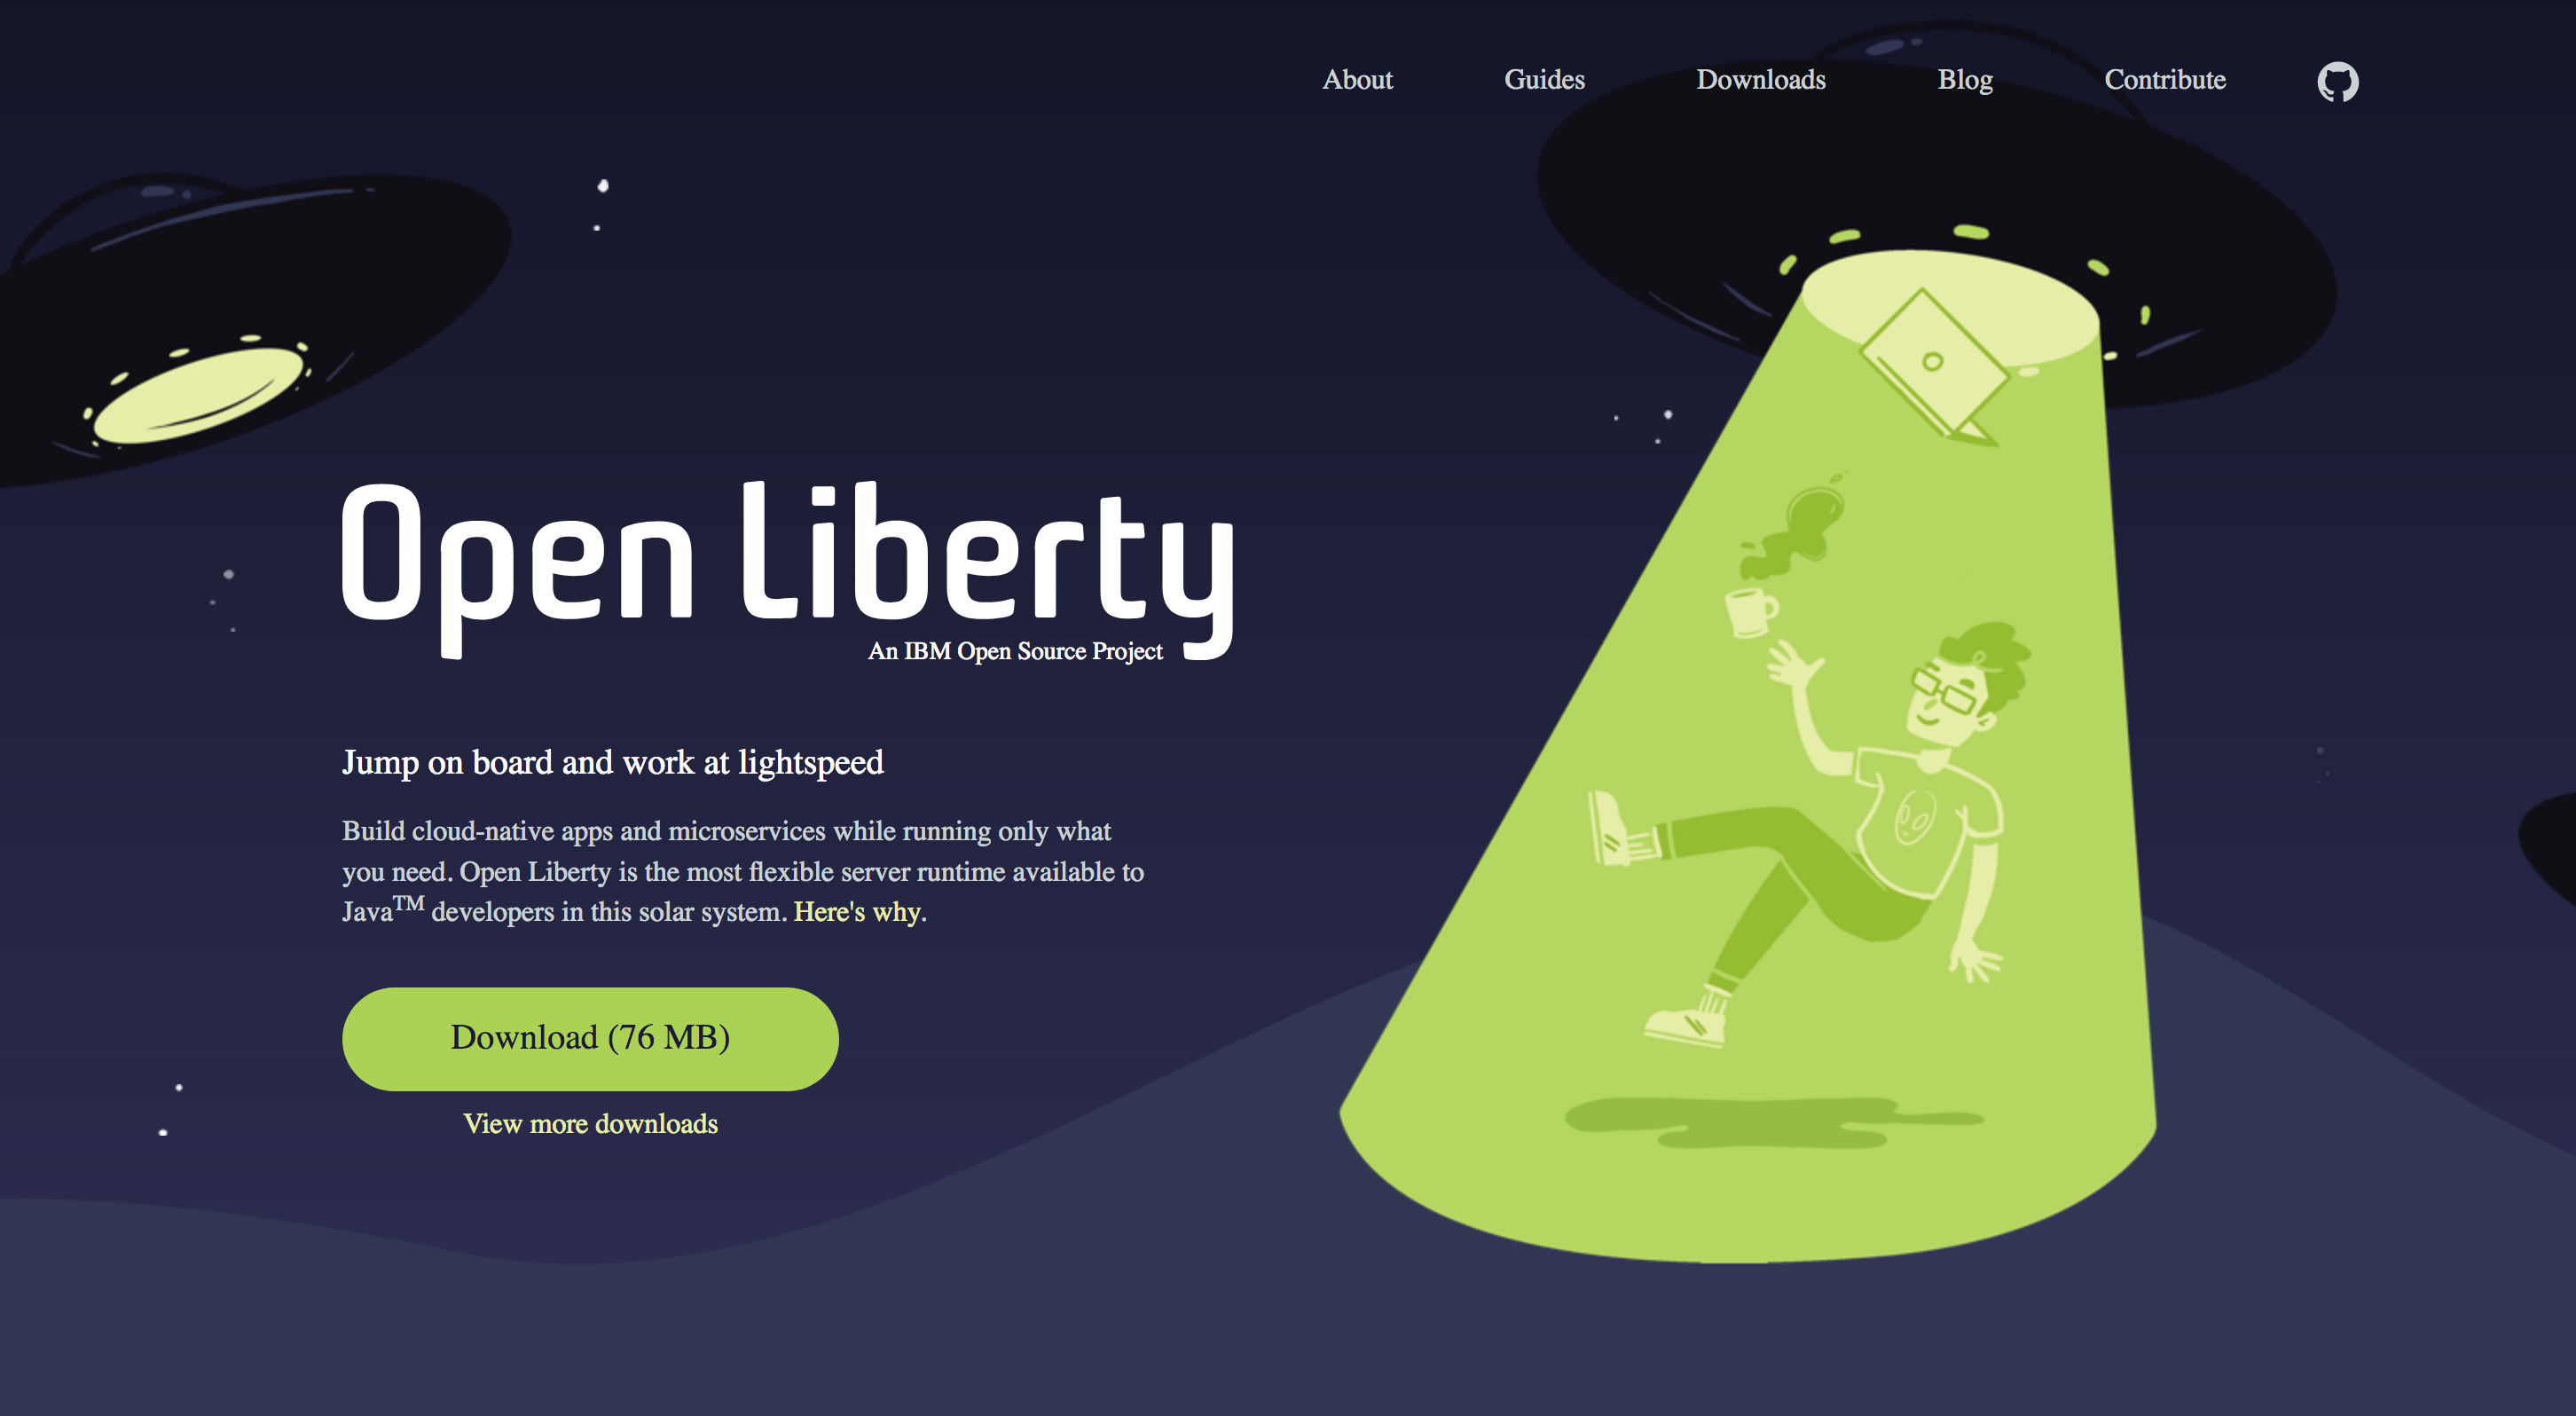
\includegraphics[width=\linewidth]{Images/liberty}
\end{figure}
\end{frame}


\begin{frame}{JavaEE 8 el ultimo gran Java EE}
\begin{figure}
	\centering
	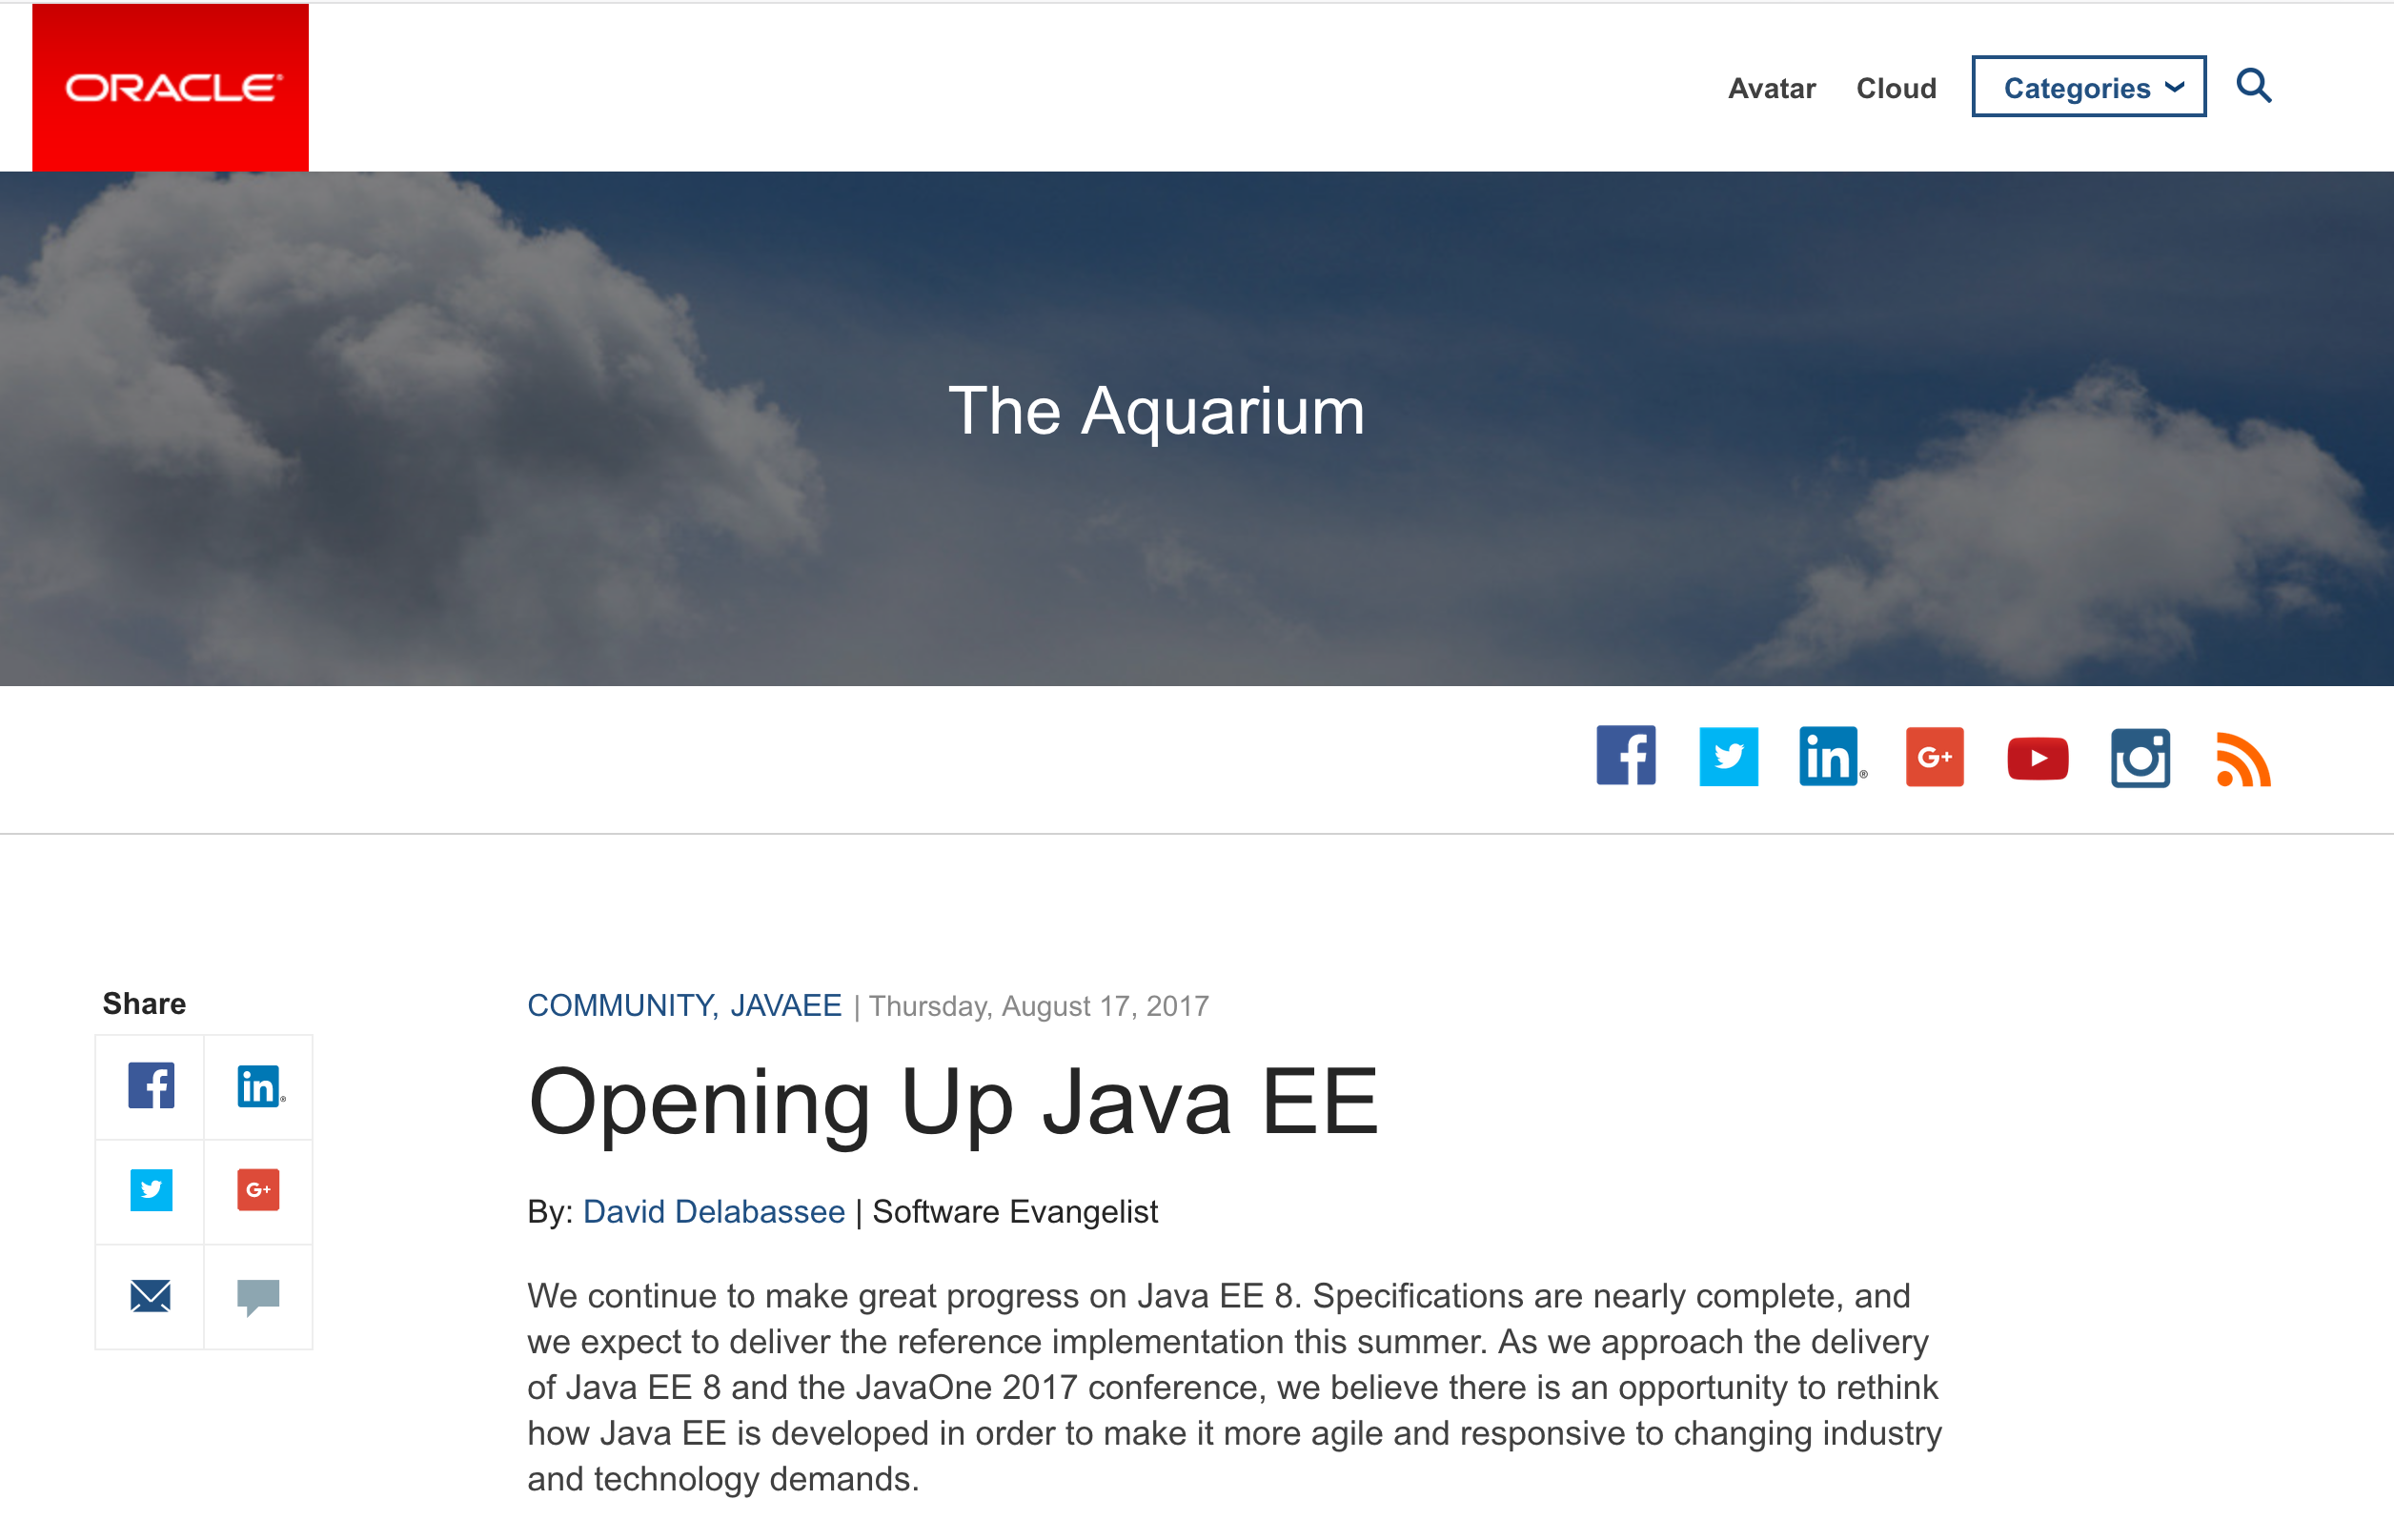
\includegraphics[width=\linewidth]{Images/javaeeopen}
\end{figure}
\end{frame}


\begin{frame}{EE4J}
\begin{figure}
	\centering
	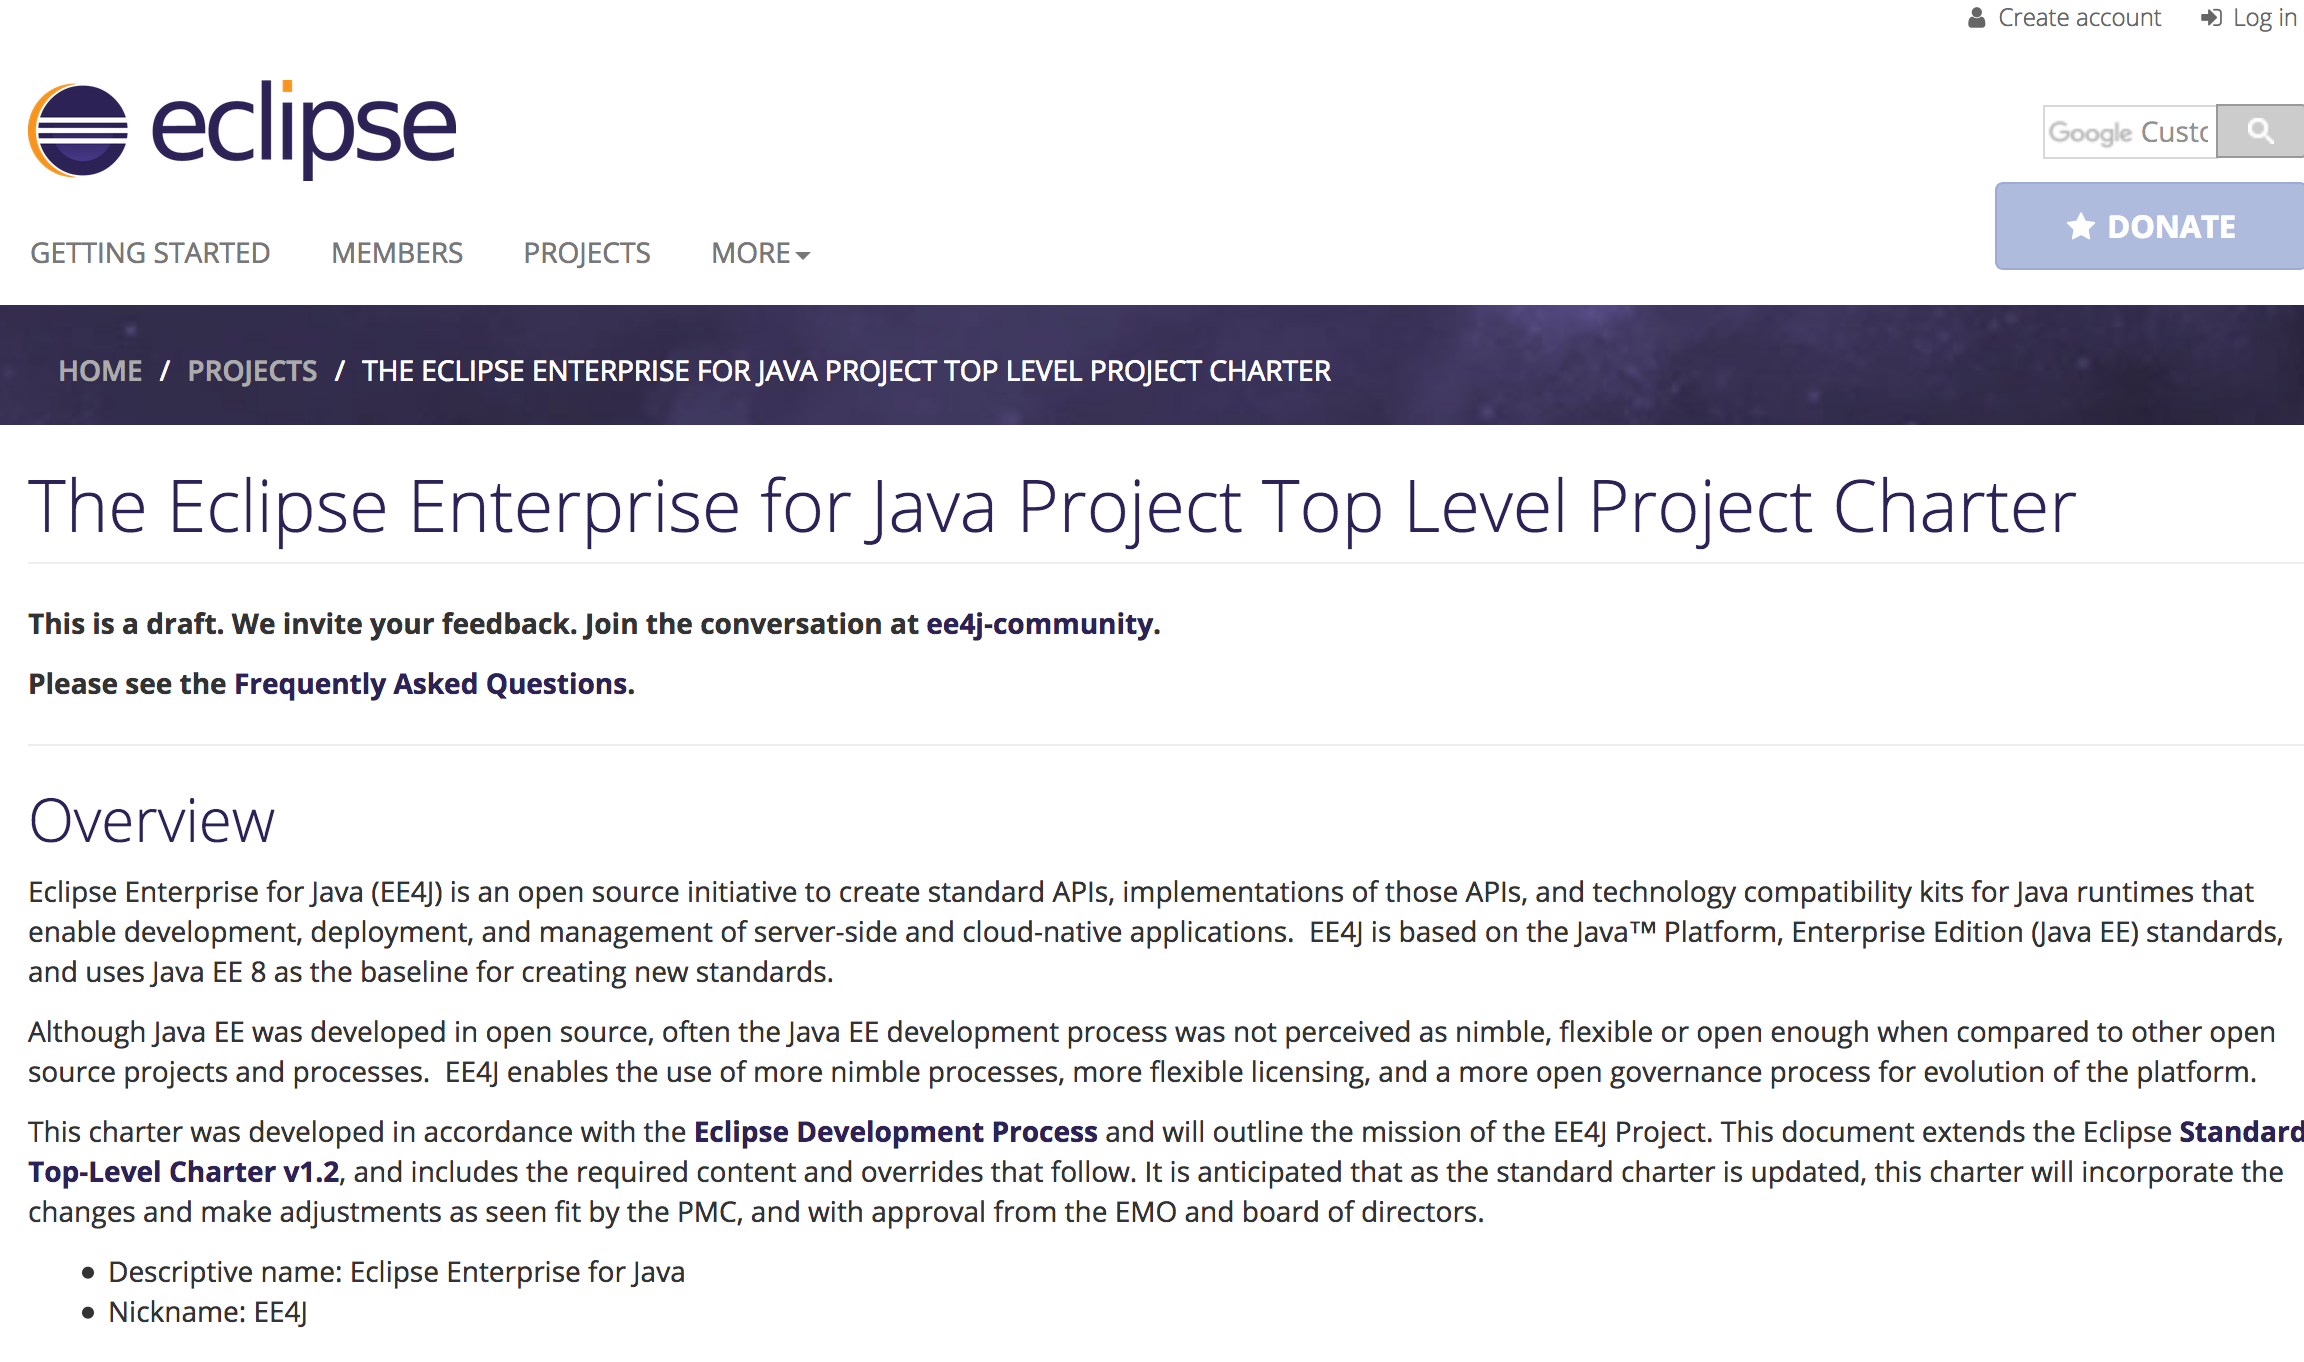
\includegraphics[width=\linewidth]{Images/ee4j}
\end{figure}
\end{frame}

\begin{frame}{Gracias}
\begin{itemize}
\item me@vorozco.com
\item \url{https://www.vorozco.com}
\item \url{http://github.com/tuxtor/slides}
\end{itemize}
\begin{center}

\includegraphics[width=0.1\linewidth]{Images/cclogo}
\\
This work is licensed under a Creative Commons Attribution-ShareAlike 3.0 Guatemala License.
\end{center}
\end{frame}
\end{document}
